\chapter{显示器的二三事}
\label{screens-and-their-secrets}

\begin{intro}
  这一章我们介绍一个\nameref{computer-and-its-components}不曾介绍过的电脑硬件——显示器。
  作为电脑与我们直接打交道的「第一线」,显示器的显示效果,直接影响着我们操作电脑的体验。
  看完这一部分,你或许能找到下面这些问题的答案:
  \begin{itemize}
    \item 为什么我的电脑屏幕看起来远没有手机 / 平板电脑那么细腻?
    \item 我喜欢画画,为什么我画出来的作品在电脑和其他设备上的颜色差距这么大?
    \item 我想选购新笔记本电脑 / 显示器,我应该关注哪些方面?
  \end{itemize}
\end{intro}

如果说眼睛是心灵的窗户,那么显示器 / 显示屏就是电脑的「心灵之窗」。
比起 CPU、内存和硬盘那些内在的配置,显示器的显示效果能够相当直观地一眼分出高低。
在这一部分,我们将介绍与显示器有关的那些事,并为大家以后选购电脑 / 显示器时提供一些参考。

\section{像素、分辨率和 PPI}

显示器上的内容是通过一个个彩色格子「拼」出来的,这样的一个小格子叫做一个「像素」或者「像素点」。
由于每个格子的颜色都可以被独立控制,我们的屏幕才得以显示各种各样的内容。

\begin{figure}[htb!]
  \centering
  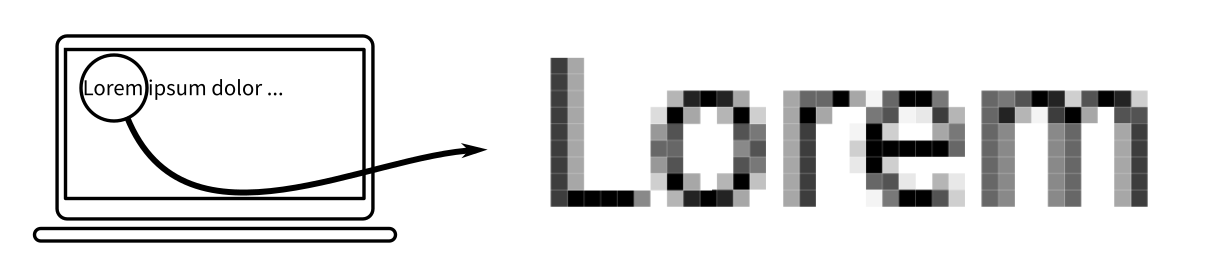
\includegraphics[width=10cm]{assets/Display.png}
  \caption{何为「显示」?}
  \label{Display}
\end{figure}

不难想象,屏幕上这样的「像素点」的个数,自然是屏幕的一个非常关键的指标。
假设现在某显示器在横向有 1920 个这样的像素点,在纵向有 1080 个这样的像素点,那么我们就把「1920 × 1080」称作是这个屏幕的「分辨率」。
顾名思义,「分辨率」影响着屏幕的「分辨」能力——分辨率越高,像素点的数量就越多,理应就有更好的「分辨」能力。

例如,假设我们有两块屏幕,它们的尺寸一样,但分辨率不同——一块屏幕分辨率高,为 1920 × 1080;
另一块低,只有 1366 × 768。如果我们让这两块屏幕显示一个同样尺寸(看起来一样大)的苹果,那么分辨率高的那块屏幕的显示效果就会更加细腻。
在屏幕尺寸相同的情况下,分辨率高的那块屏幕能拿出更多的像素点来「拼」出图像,自然「马赛克」感就要弱上许多。

\begin{figure}[htb!]
  \centering
  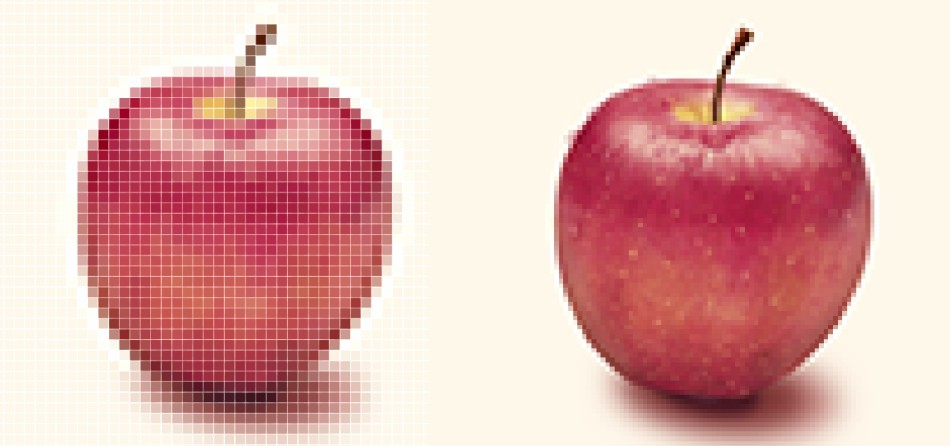
\includegraphics[width=8cm]{assets/Different_Apple.jpg}
  \caption{不同的屏幕,同样的苹果}
  \label{Different_Apple}
\end{figure}

但是,如果两块屏幕的尺寸不一样呢?假设一块屏幕分辨率高,但它尺寸也大;另一块屏幕分辨率低,可是它尺寸很小。
前者尽管有更多的像素点,可是由于屏幕尺寸变大了,像素点的「分布」依然会变得稀疏;
后者尽管像素点数量少,可是屏幕尺寸小,也许像素点看起来还更加密集呢!
这么看来,单凭一个分辨率,我们并不能直接就推断出谁的显示细腻,谁的显示粗糙。

为了公平地衡量屏幕显示的细腻程度,我们不再关注整个屏幕上的像素点的多少,而是关注屏幕在一定尺寸上像素点的多少。
具体地,我们用屏幕在 1 英寸(等于 2.54 厘米)这个长度上的像素点的个数来衡量它的显示细腻程度,这个数字称为「每英寸像素数」(pixels per inch,简称「PPI」)。
PPI 由「屏幕分辨率」和「屏幕尺寸」两个因素决定,可以通过简单的数学计算算出来。

现在,请你仔细观察你的电脑的屏幕和手机的屏幕。直观上,手机的屏幕要显得细腻得多——对着电脑屏幕凑近看,你或许能看出像素点之间的边界;
但对着手机屏幕,你很难再感受到那种锯齿感。
这就是因为手机屏幕的 PPI 远高于电脑屏幕造成的。
在今天,手机屏幕和电脑屏幕的分辨率相差不大,平均是在「两千上下乘以一千上下」这个水平;
但手机屏幕比电脑的小得多,PPI 因此可以达到电脑的数倍,观感自然就比电脑要好得多了。

\section{色域、色准和面板类型}

接下来,我们聊一聊屏幕的「色彩」。
屏幕的色彩体验由很多因素决定,这里我们主要介绍「色域」、「色准」以及面板类型。

\subsection{色域}

首先我们简单介绍一下「色域」。
人眼能够识别的全部色彩,可以以数学和光学的方式进行一定程度的刻画。
图 \ref{CIE1931xy_blank} 展示的图形称为「CIE 1931 色彩空间」,可以理解成我们人眼能够分辨的所有颜色构成的集合。

人眼的色彩分辨能力非常强大,而以我们目前的科学技术,是造不出能够显示出所有这些颜色的显示屏的。
因此,人们在研究人眼对不同颜色的敏感程度后,从这个色彩空间中「划」出一部分子空间,用这样的子空间来指导我们生产显示器、照相机等色彩产品。
例如,图 \ref{NTSC_sRGB} 中的黑色和蓝色的两个三角形,就是两种不同的划法——一种称为「NTSC」,一种称为「sRGB」。

\begin{figure}[htb!]
  \begin{minipage}{6.5cm}
    \centering
    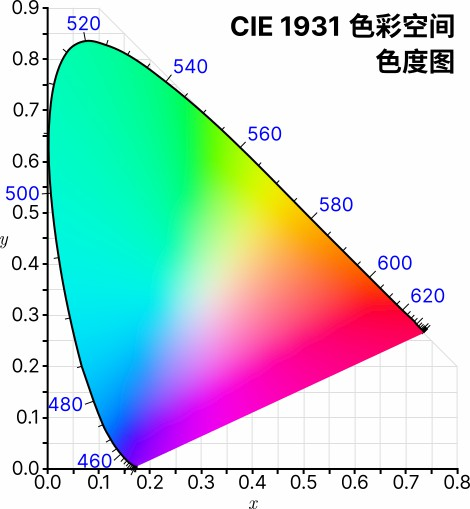
\includegraphics[width=6cm]{assets/CIE1931xy_blank.jpg}
    \caption{CIE 1931 色彩空间色度图}
    \label{CIE1931xy_blank}
  \end{minipage}
  \qquad
  \begin{minipage}{6.5cm}
  \centering
  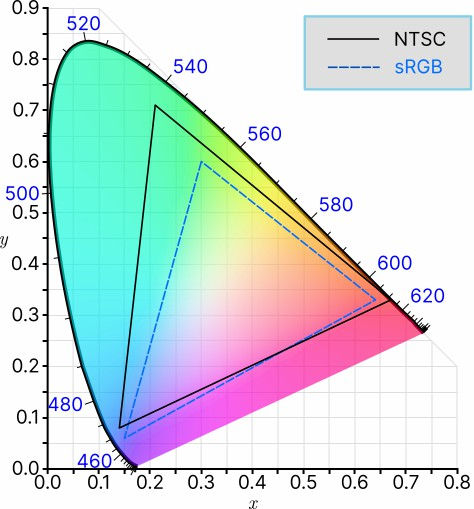
\includegraphics[width=6cm]{assets/NTSC_sRGB.jpg}
  \caption{NTSC 与 sRGB 色彩空间}
  \label{NTSC_sRGB}
  \end{minipage}
\end{figure}

然而,在这样的子空间之上,受限于成本等因素,人们发现在生产显示器时,还可以进一步「减配」——毕竟并不是所有人都要求屏幕能显示出这么多绚丽的颜色,对吧?
例如,在上面的「NTSC」色彩空间之上,再进一步划出更小的区域,用这样的小区域作为显示器色彩的标准。
例如,将 NTSC 色域的 45\% 和 72\%「拎出来」,就得到了两套更小的色彩空间:

\begin{figure}[htb!]
  \centering
  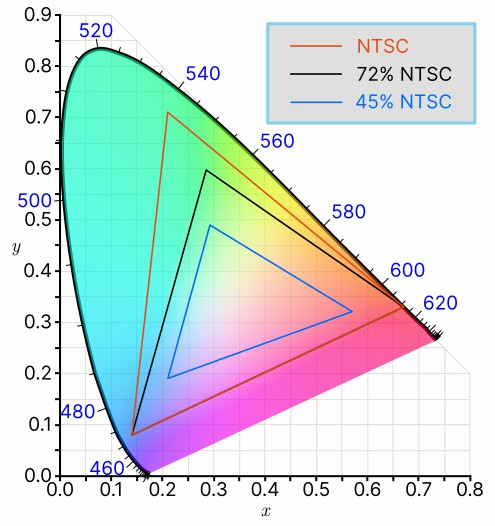
\includegraphics[width=6cm]{assets/NTSC_72_45.jpg}
  \caption{NTSC 与其子空间}
  \label{NTSC_72_45}
\end{figure}

如果某款显示器能够展现出 45\% 的 NTSC 颜色,我们就称这款显示器的「色域」是 45\% NTSC,民间有时简称 45\% 色域。
同样地,如果某显示器能展现 72\% 的 NTSC 颜色,我们就称它是 72\% 色域。
目前来说,45\% 色域又被称为是「低色域」,72\% 及以上的色域都能够统称为「高色域」。
尽管看上去 45\% 色域小得吓人,但在实际生活使用中,它也是基本足够的——除非你眼睛比较敏感,否则一眼不容易看出 45\% 色域和 72\% 色域的具体差别。
不过,如果你有进行艺术创作等的需求,或者单纯追求更舒适的体验,那么一块高色域的屏幕对你来说是非常必要的。

\begin{figure}[htb!]
  \centering
  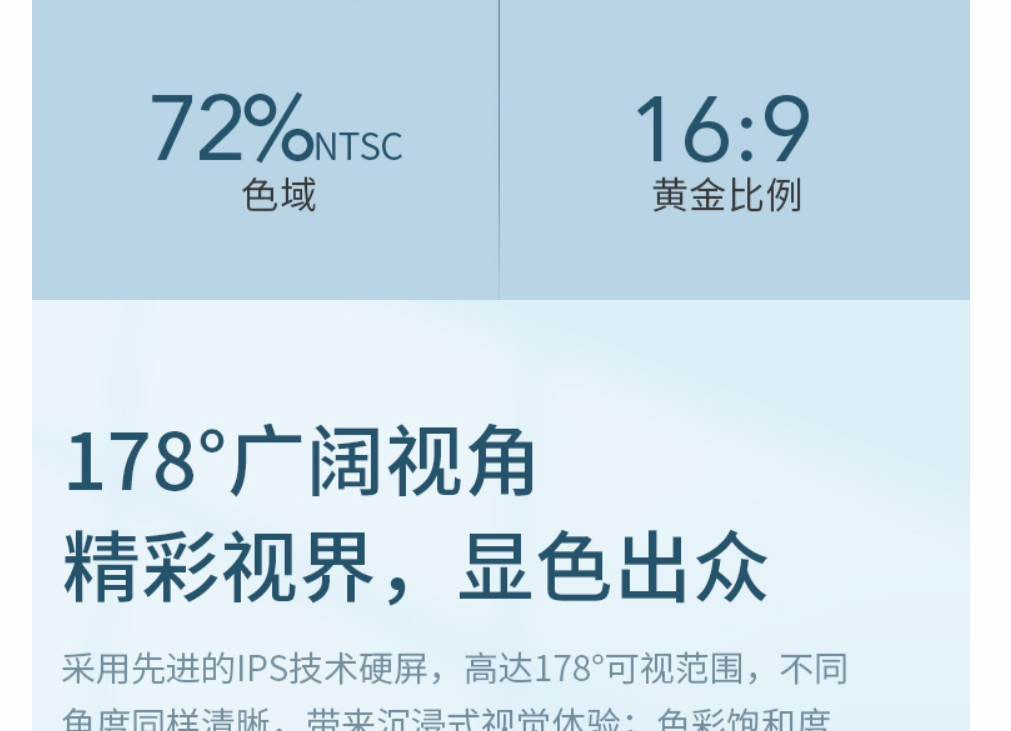
\includegraphics[width=7cm]{assets/72_NTSC_Ad.jpg}
  \caption{宣传 72\% NTSC 色域的屏幕}
  \label{72_NTSC_Ad}
\end{figure}

除了用 NTSC 色域作为参考来「划」色域之外,现在很多厂商还会用上文中提到的另一个色彩空间 sRGB 来作为参照。
sRGB 的覆盖范围较 NTSC 小些,但它是今天使用得更普遍、更广泛的设计标准;相比之下,NTSC 则是一个老旧的电视机标准。
从色域面积上来说,sRGB 99\% 的覆盖率和 NTSC 72\% 的覆盖率基本相当,因此 sRGB 99\% 甚至更高的显示器同样是「高色域」的显示器,都能带来非常不错的体验,不过要说明的是:99\% sRGB 并不等同于 72\% NTSC。

\begin{figure}[htb!]
  \centering
  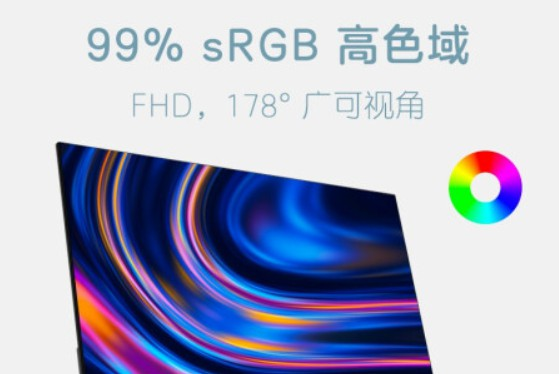
\includegraphics[width=7cm]{assets/99_sRGB_Ad.jpg}
  \caption{宣传 99\% sRGB 色域的屏幕}
  \label{99_sRGB_Ad}
\end{figure}

除了 NTSC 和 sRGB 之外,还有诸如 DCI-P3 这样的更大、更专业的色彩空间,现在许多民用显示器也开始以「DCI-P3 90\%」作为自己的卖点。这里我们不再赘述相关的细节,有兴趣的读者可以自行上网查阅资料。

\subsection{色准}

如果说色域决定了显示器色彩的上限,那么色准则影响着显示器的实际体验。
顾名思义,「色准」就是「色」的「准确」程度。下面是一个极端的例子:某显示器能显示 100 万种颜色,但是这 100 万种颜色的对应关系都是错的——红色会显示成绿色,蓝色会显示成紫色……那么这台显示器的体验必然是相当糟糕的。
这种色彩还原的准确程度,我们就称为一个显示器的色准。

\begin{figure}[htb!]
  \centering
  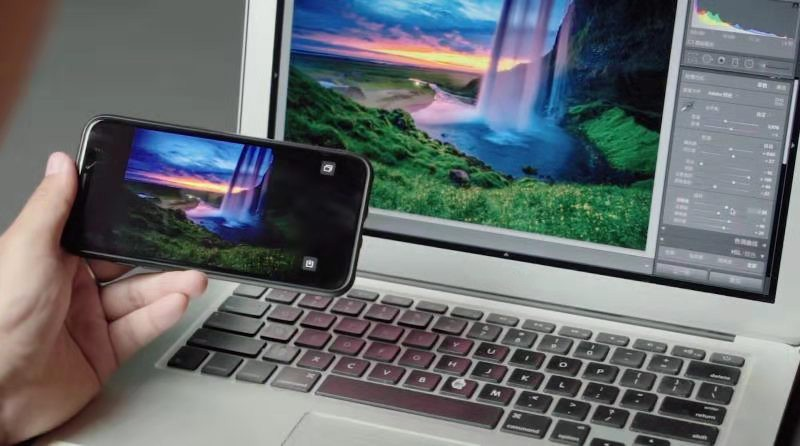
\includegraphics[width=8cm]{assets/Off_Color.jpg}
  \caption{色差}
  \label{Off_Color}
\end{figure}

将一张相同的图片分别在电脑、手机、平板电脑等多台设备上同时打开,再将它们并排放在一起,有时你会发现不同设备之间的色彩差异巨大。这就是「色准」的差异。
每个设备都「有着自己的想法」,对于同一个颜色的显示表现各不相同。
如果你希望自己的作品能够尽量真实地反映出颜色,那么色准将是你在选择屏幕时必须考量的因素。

色准的衡量是通过「距离」来衡量的:我们让显示器显示某个颜色 A,但显示器实际显示出来的是颜色 A*,A 和 A* 两个颜色在色彩空间图上的「距离」就能反映出这台显示器对颜色 A 的准确程度。
如果让显示器显示一系列常用的标准色,并计算各个颜色「距离」的平均值,就可以反映出一台显示器的色准水平。
具体在产品上,厂家往往用「Delta E」($\Delta E$)这个参数来描述这样的距离。
平均 Delta E 的值越小,显示器的色彩就越精准。下面是某品牌显示器的商品介绍,厂商宣称 Delta E < 2,这已经是相当高的色准了。

\begin{figure}[htb!]
  \centering
  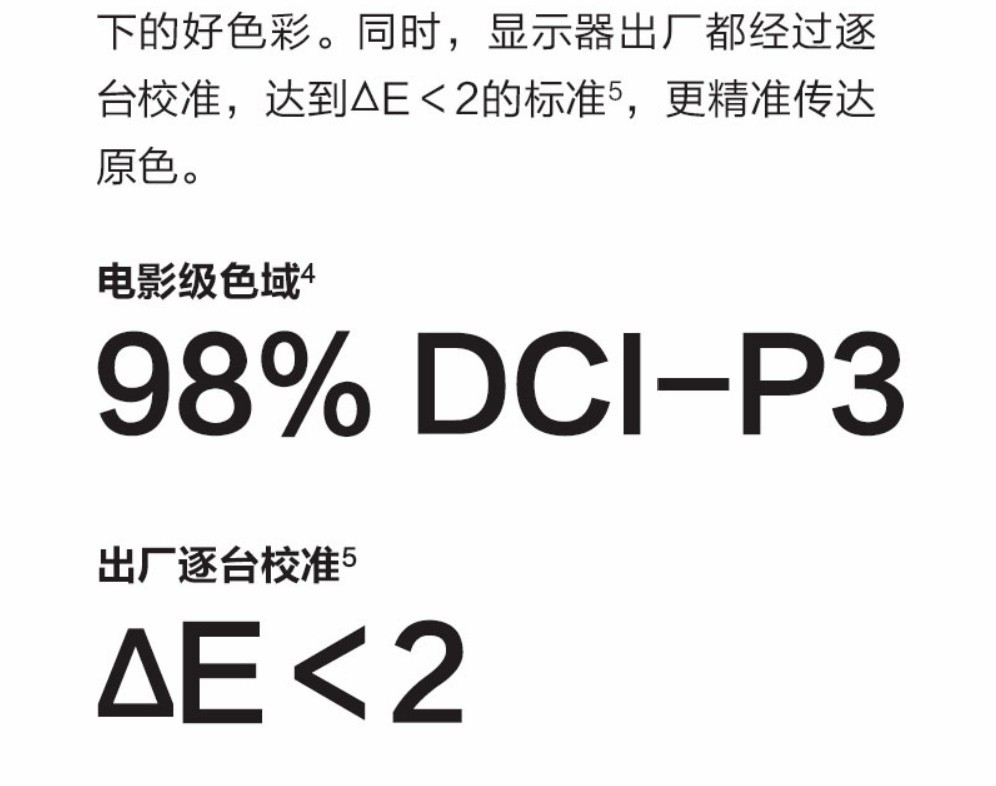
\includegraphics[width=7cm]{assets/Delta_E_below_2.jpg}
  \caption{Delta E < 2 的宣传}
  \label{Delta_E_below_2}
\end{figure}

与色域不同,色准是可以在显示器出厂后再次提升的,提升色准的过程叫做「校色」。
校色需要使用专门的设备「校色仪」,搭配专门的软件来进行。
校色的原理可以理解成重新调整显示器的显示颜色和实际颜色之间的对应关系,从而消除颜色显示的偏差。

除了购买显示器后人工校色外,一些显示器和笔记本电脑在出厂时会进行「逐台校色」,以提升显示器的出厂色准。
这也是厂商喜欢用来宣传的一个卖点。

\subsection{面板类型}

在今天,我们大多数人的电脑屏幕都是使用的液晶显示屏(LCD)。
液晶显示屏根据「面板类型」的不同,在观感上有着很大的差异。
目前,常见的面板类型有 TN、IPS 和 VA 三种,下面我们分别介绍这三种面板在色彩方面的区别。

\begin{itemize}
  \item TN 面板的显示屏(简称 TN 屏)在色彩方面表现最差。
    这种屏幕的「可视角度」非常小、而且普遍存在色彩泛白的问题。
    所谓「可视角度」小,表现在当你的视线没有正对着屏幕时,看到的颜色就有非常大的偏差。
    所谓的「色彩泛白」,可以参看图 \ref{IPS_vs_TN}。
    \begin{figure}[htb!]
      \centering
      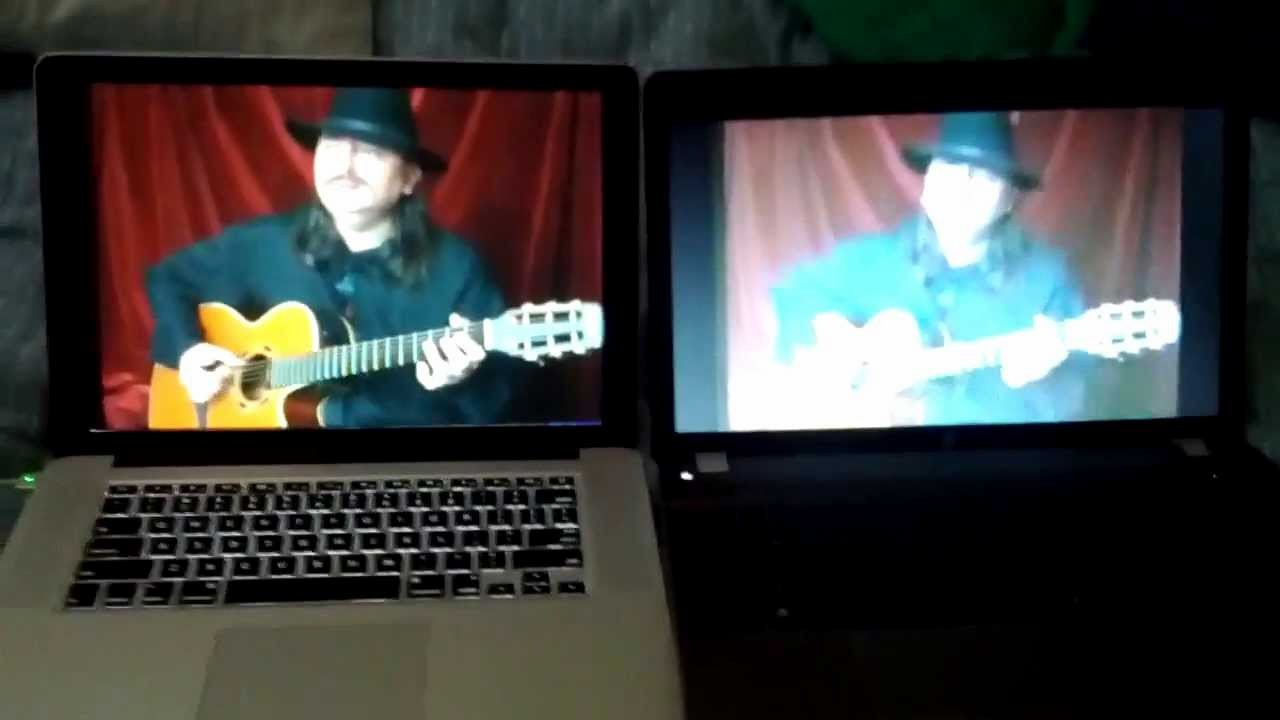
\includegraphics[width=11cm]{assets/IPS_vs_TN.jpg}
      \caption{IPS屏幕(左)与TN屏(右)}
      \label{IPS_vs_TN}
    \end{figure}\\
    TN 屏是一种色域和色准都不好的屏幕。它曾经很常用,如今则主要用在低配置的显示器和笔记本上。
    尽管目前厂商也在不断改善 TN 屏的色彩,但在今天,如果你对屏幕色彩方面的观感有一定要求,那么 TN 屏都不会是你的选择。
  \item IPS 面板的显示屏(IPS 屏)在色彩方面表现相当出色。
    一方面,IPS 屏可以做到很高的色域;
    另一方面,IPS 屏有着接近于 180° 的「可视角度」——换句话说,IPS 屏无论从哪个角度看,色彩都是趋于一致的。
    这也是厂商总是会将 IPS 屏作为一个「卖点」的原因。
    在过去,IPS 屏的成本远远高于 TN 屏,因此只在高端的笔记本和显示器上使用;
    但现在,随着科技的进步,越来越多的中低价位产品也开始配备 IPS 屏幕了。
    \begin{figure}[htb!]
      \centering
      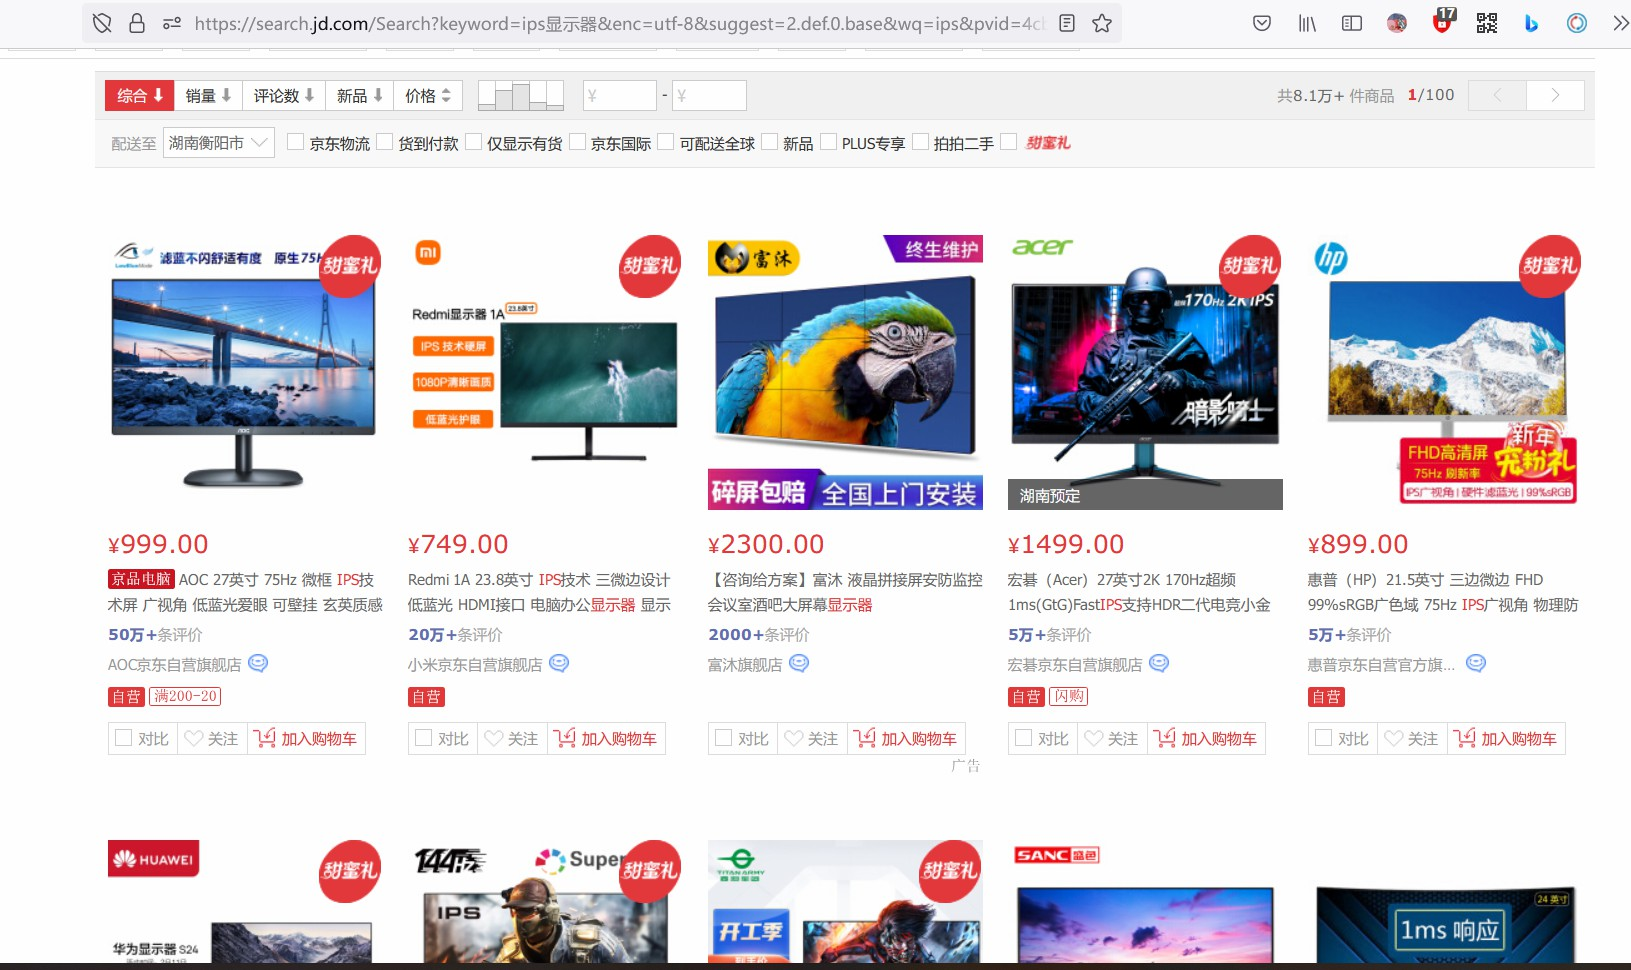
\includegraphics[width=13cm]{assets/IPS_at_Low_Price.jpg}
      \caption{市面上一些中低价位IPS屏幕}
      \label{IPS_at_Low_Price}
    \end{figure}\\
    当然,同样是 IPS 屏幕,它们仍然有色域和色准的区别。
    换言之,我们的比较必须是多维度的:总体上,IPS 屏幕的观感好于 TN 屏;
    高色域的 IPS 屏幕的观感好于低色域的 IPS 屏幕;色准好的 IPS 屏幕观感好于色准差的屏幕。
  \item VA 面板的显示屏(VA 屏)也是一种色彩相当优秀的屏幕。
    VA 屏由于技术上更容易做大、做宽,而且还可以做成曲面,同时价格没有 IPS 那么高,因此市面上的很多低价「带鱼屏」「曲面屏」都在使用 VA 面板。
    VA 面板的缺点主要是拖影比较严重,因此在某些程度上不是十分适合游戏。
    下图是某品牌千元级的「带鱼屏」产品,使用的就是 VA 面板。
    \begin{figure}[htb!]
      \centering
      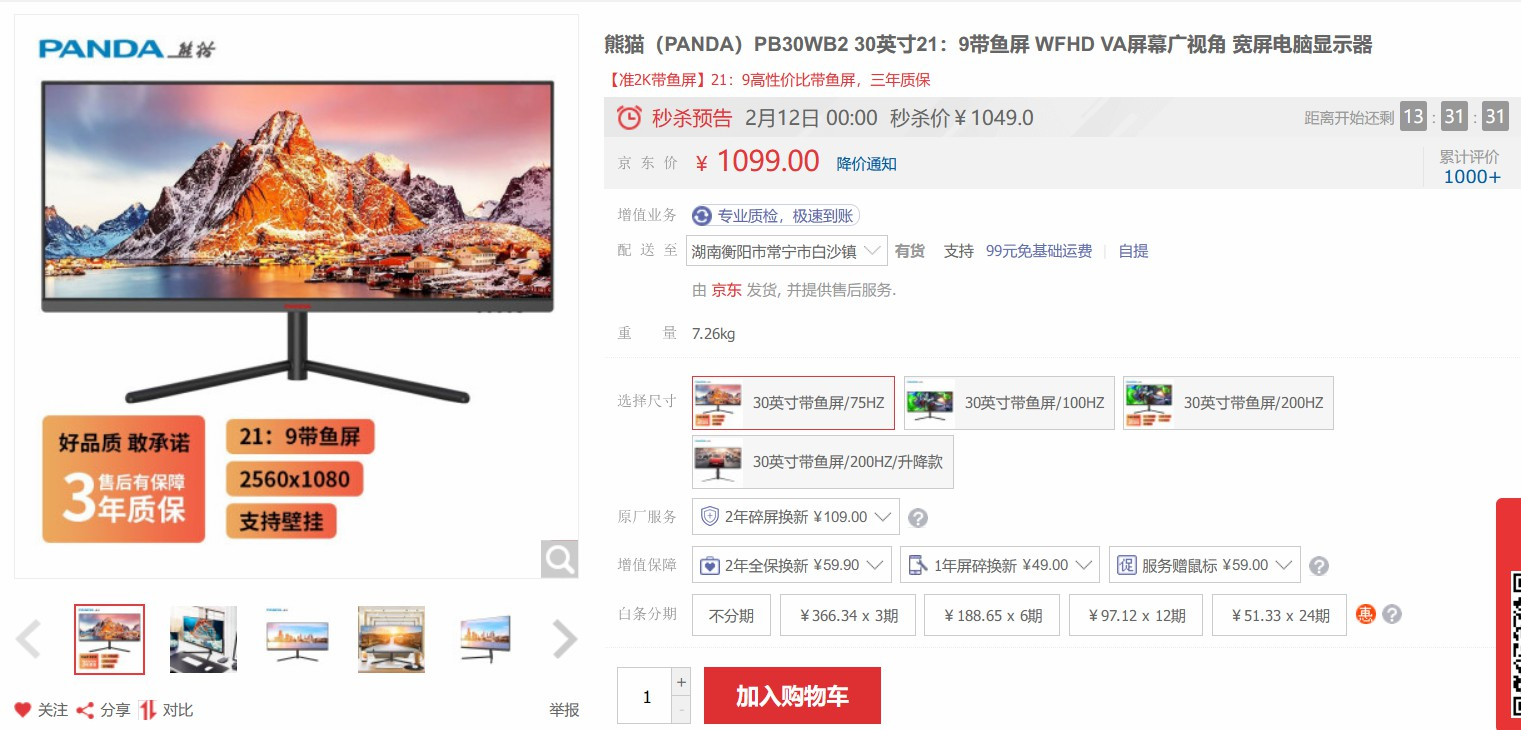
\includegraphics[width=11cm]{assets/VA_at_Low_Price.jpg}
      \caption{千元VA「带鱼屏」}
      \label{VA_at_Low_Price}
    \end{figure}\\
    VA 面板是一种色彩优秀的高性价比选择。
    如果你不怎么玩游戏,但又喜欢「大屏」「宽屏」「曲面屏」,那么一众 VA 屏可能就是你的意中「屏」。
\end{itemize}

\section{刷新率}

也许你已经知道,显示器是利用人眼的视觉暂留效应,将一张张的静态画面「拼」成动态画面并展示给我们看的。
然而,显示器不可能做到「拼」的速度无限快,每秒钟换几十张已经是很多显示器的极限。
这个「每秒钟换几十张」就是显示器的刷新率,它的单位是赫兹(Hz)。
例如,60 Hz 的显示器,它每秒钟最多能向我们展示 60 个画面;而 120 Hz 的显示器,则每秒可以展示 120 个。

\begin{figure}[htb!]
  \centering
  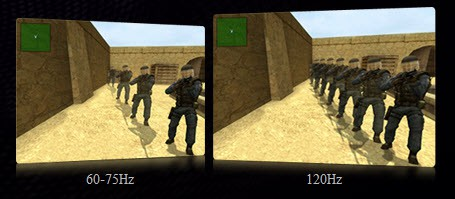
\includegraphics[width=8cm]{assets/60Hz_vs_120Hz.jpg}
  \caption{不同刷新率的对比}
  \label{60Hz_vs_120Hz}
\end{figure}

如果你是游戏玩家,那你自然会知道「帧率」这个概念。
帧率是电脑每秒可以生成的画面的个数,而刷新率是显示器每秒能够显示的画面的个数。
最理想的情况下,帧率和刷新率相等,这样电脑生成的每一张画面都能完美地被显示器展现。
如果帧率很高,但刷新率不够,那么就会有许多张画面没能够被显示——显示器跟不上画面来的速度;
如果帧率低,而刷新率高,那么显示器就会在多次显示同一帧。
这两种情况都会造成一个恶性后果:画面有「撕裂」感。
诸如「垂直同步」「FreeSync」之类的选项可以避免这两种情况带来的画面撕裂,具体细节请读者自行上网查找。

在今天,大多数办公用的笔记本和显示器的刷新率都是 60 Hz 或 75 Hz。
一些游戏本和游戏显示器的刷新率则能达到 120 Hz、144 Hz 甚至更高。
更高的刷新率能带来更流畅的游戏体验(前提是,你的配置足够好,能够到达这么高的帧率),但也意味着更高的价格。
如果你是游戏玩家,那么这将是你需要考虑和进行取舍的一个因素。

\section{总结}

在文章的最后,我们为大家总结一下选购显示器时的关注点:

\begin{enumerate}
  \item 分辨率和尺寸:想要更加「细腻」的显示效果,\regcolor{在尺寸相同的条件下选分辨率高的}。
    比如,13 寸的笔记本屏幕,分辨率最好在 1920 × 1080 以上;21 寸的台式机显示器,分辨率最好在 2560 × 1440 以上。
  \item 色域与色准:若对色彩有要求,\regcolor{选择「DCI-P3 90\%」「100\% sRGB」「99\% sRGB」「72\% NTSC」等高色域}的显示器;
    对色准有要求,选择厂商\regcolor{宣称「出厂校色」并且 Delta E 比较小}(例如,Delta E < 2)的显示器。
  \item 面板类型:\regcolor{选择 IPS 屏幕或者 VA 屏幕。}
    TN 屏非常「瞎眼」,除非你知道自己在做什么,否则不要选择。
  \item 刷新率:若你\regcolor{追求游戏性能,在配置(尤其是显卡)足够的情况下,选择 144 Hz、120 Hz 等高刷新率}的;
    反之,60 Hz、75 Hz 和 90 Hz 的显示器已经足够满足你的需求。
\end{enumerate}

\practice

\begin{enumerate}
  \item 查看你电脑显示器的分辨率。可以通过在桌面上右键 →【显示设置】→【显示分辨率】来查看。
  \item 了解你电脑显示器的尺寸。尺寸指的是屏幕对角线的长度,一般单位是「英寸」(inch)。然后,结合上一题查到的分辨率,计算你屏幕的 PPI。
  \item 在电商平台上查找显示器 / 笔记本电脑,看看厂商有没有宣传屏幕的色域、色准和刷新率信息。
\end{enumerate}